% !TEX root = 15cvpr.tex

\section{The Proposed Model}

\begin{figure*}[htb]
    \begin{center}
        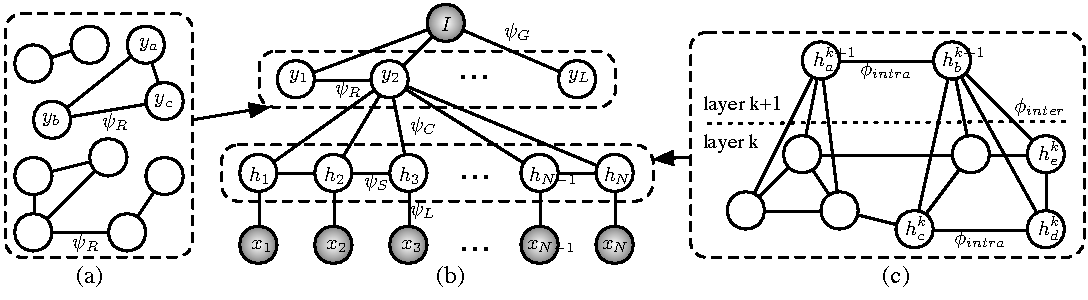
\includegraphics[width=0.9\linewidth]{graphmodel.pdf}
    \end{center}
    \vspace{-3mm}
    \caption{Graphical representation of our model, shadow nodes are observed variables and blank nodes are latent variables. (a) shows the learnt label correlations. (b) represents the joint inference framework. (c) shows the hierarchical model and spatial constraints.}
    \label{fig:graphmodel}
\end{figure*}

We formulate the semantic segmentation problem as a CRF over image superpixels incorporating various contextual relations, for instance, the associations between high-level semantic concepts and low-level visual appearance, inter-label correlations, spatial neighborhood cues, and the label consistency between image-level and pixel-level.

%a set of weakly labeled social images are denoted as $\mathcal{I}=\{I_k\}_{k=1}^N$, where $N$ is the total number of  images.

More formally, suppose that each image $I$ is associated with a label vector $\boldsymbol{y} = [y_1,...,y_L]$, where $L$ is the number of categories, and $y_i=1$ indicates that the $i$-th category is present in this image, otherwise $y_i=0$. In the training set, $\boldsymbol{y}$ is given; however, it may be incorrect or incomplete. In the test set, $\boldsymbol{y}$ is unknown.
For each image, we employ the existing multi-scale segmentation algorithm and get a set of superpixels   $\{x_p\}_{p=1}^M$ over multiple quantization levels.
Here, $M$ is the total number of superpixels in image $I$.
The label of superpixel $x_p$ is denoted as $h_p\in \{1,2,...,L\}$, and the labels of all superpixels for image $I$ are $\boldsymbol{h}=[h_1,...,h_M]$, which are not provided in training/test stage.

Our goal is to infer the most suitable semantic label for each superpixel in an image and the adjacent superpixels sharing the same semantic label are fused as the whole one.
In order to achieve this, we build a CRF on the image-level label variables $\boldsymbol{y}$ and the superpixel-level label variables $\boldsymbol{h}$.
We connect each superpixel variables to its neighbors to encode a local smoothness constraint.
Specifically, let $\mathcal{N}$ denote the neighborhood system among the superpixels, we define an energy function $E$ with five types of potential as follows:
\begin{equation}
    \label{eq:energyfunction}
    \begin{aligned}
        E(\boldsymbol{y},\boldsymbol{h},\boldsymbol{I}&) = \sum_{i=1}^L{\varphi_{i}(y_i,\boldsymbol{I})}
                            + \sum_{1 \le i,j \le L} {\varphi_{ij}(y_i,y_j)}\\ &+ \sum_{p=1}^M{\psi_{p}(h_p,\boldsymbol{x_p})}+ \sum_{(p,q) \in \mathcal{E}}{\psi_{pq}(h_p,h_q)}\\ &+ \tau (\boldsymbol{y},\boldsymbol{h})
    \end{aligned}
\end{equation}
where $\varphi_{i}$ and $\psi_{p}$ encode the unary potential of image-level and superpixel-level constraints respectively, $\varphi_{ij}$ impose label correlation and co-occurrence, $\psi_{pq}$ are the spatial context constraints for each superpixel, and $\tau$ ensure the consistency between global and regional labels.
The posterior distribution $P(\boldsymbol{y},\boldsymbol{h}|\boldsymbol{I})$ of the CRF can be written as $P(\boldsymbol{y},\boldsymbol{h}|\boldsymbol{I}) = \frac{1}{Z(\boldsymbol{I})}\exp{\{-E(\boldsymbol{y},\boldsymbol{h},\boldsymbol{I})\}}$, where $Z(\boldsymbol{I})$ is the normalizing constant.
Thus, the most probable labeling configuration $\boldsymbol{y}^{\star},\boldsymbol{h}^{\star}$ of the random field can be defined as  $\boldsymbol{y}^{\star},\boldsymbol{h}^{\star} = \arg \min_{\boldsymbol{y},\boldsymbol{h}} E(\boldsymbol{y},\boldsymbol{h},\boldsymbol{I})$.
The details of each potential will be described in the following sections, and a graphical representation of the energy function is illustrated in Figure \ref{fig:graphmodel}.


\subsection{Unary Potential}
\textbf{Image-Level Potential}
We model input image by two aspects: On the one hand, we utilize CNN to represent the appearance model of each image, especially the first fully-connected layer containing 4096 neurons of a 19-layers model \cite{simonyan2014very}.
On the other hand, for latent semantic concept model, we model the CNN representation as a finite mixture of latent semantic concepts by pLSA \cite{sivic2005discovering}, which can recover visual models of semantic labels in a completely unsupervised manner.
Similar to \cite{wang2014weakly}, we regard fully-connected layer as input considering each neuron as a visual word $w_i$ and each image as a document $d_j$, then the occurrence frequency of image on $w_i$ is the i-th dimension of $d_j$.
In addition, there is a hidden semantic topic variable $t_k$ associated with all the visual words.
We treat each topic $t_k$ as a latent semantic concept. The pLSA optimizes the joint probability $P(w_i,d_j,t_k)$.
Marginalizing over the latent concept $t_k$ determines the conditional probability $P(w_i|t_k)$:
\begin{equation}
  P(w_i|d_j) = \sum_{k=1}^K{P(t_k|d_j)P(w_i|t_k)}
\end{equation}
where $P(t_k|d_j)$ is the probability of latent semantic concept $t_k$ occurring in image $j$.
Formally, we formulate image-level feature as $\boldsymbol{I}$ by concatenating the appearance feature $d_j$ and latent semantic concept distribution $P(\boldsymbol{t}|d_j)$, and define the $i$-th image-level label presence/absence potential $\varphi_{i}$ as follows:
\begin{equation}
    \varphi_{i}(y_i=l,\boldsymbol{I}) = -\log f_{i}^l(\boldsymbol{I})
    \label{eq:global}
\end{equation}
where $f_{i}^l(\boldsymbol{I})$ is the linear support vector machine score function associated with label $i$ for state $l \in \{0,1\}$.

\textbf{Superpixel-Level Potential}
Similar with image-level potential, we both consider the appearance model and latent semantic concept model in order to narrow down the gap between low-level feature space and high-level semantic space, in the meantime, to reduce the negative impact of inaccurate image-level labels.
Formally, let $\boldsymbol{x_p} = (\boldsymbol{a_p},\boldsymbol{c_p})$ indicates the appearance feature and latent semantic concept distribution vectors extracted from the superpixels, we encode the unary potential of superpixel-level as follows:
\begin{equation}
    \begin{aligned}
        \psi_{p}(h_p=l,\boldsymbol{x_p}) = - \log \big\{ w_1 \boldsymbol{a_p^\top}\boldsymbol{\theta_a^l}
        + w_2 \boldsymbol{c_p^\top}\boldsymbol{\theta_c^l} \big\}
    \end{aligned}
    \label{eq:local}
\end{equation}
where $\boldsymbol{\theta_a^l}, \boldsymbol{\theta_c^l}$ donate the parameters for state $l \in \{1,2,...,L\}$ with respect to appearance model and latent semantic concept model, $w_1,w_2$ are the weighting coefficients for the unary terms.
The details of learning $\boldsymbol{\theta_a}$ and $\boldsymbol{\theta_c}$ will be illustrated in Section \ref{learningparameters}.

\subsection{Pairwise Potential}

\textbf{Label Correlation}
We model inter-label co-occurrence by constructing inter-label correlation matrix which characterizing the interaction between semantic concepts and helps to model the relationship among feature space of superpixels.
Due to the unknown semantic annotation of superpixels, learning these latent information is an unsupervised learning problem.
Moreover, the context contain some useful latent information which can be learned for semantic label noise reduction.

Here we consider two aspects to construct inter-label matrix, on the one hand, we construct co-occurrence matrix $A$ to capture the inter-label correlation. $A$ is an $L \times L$ symmetric matrix and its entry $A(i,j)$, measuring the co-occurrence of concepts pair $(i,j)$ based on statistics, can be defined as follows:
\begin{equation}
    A(i,j) = 1-(1-P(i|j))(1-P(j|i))
\end{equation}
where $P(i|j)$ is the empirical probability of concept $i$ occurring under the condition that concept $j$ has occurred.

On the other hand, we determine the inter-label correlation via visual contextual cues. Here, we capture such visual cues by calculating the intersection-over-union (IoU) overlap of discriminative regions between concepts pair. The discriminative region of concept indicates the most informative sub-windows of each image within a multi-class classification framework.
The basic idea is to analyze the variation of classification score when artificially removing different regions of the image, which means to black-out specific area of raw image. We observe that discarding a discriminative sub-window causes a massive confusion for one-vs-one classifier, especially in cluster condition.

Then we produce a set of sub-windows, which are deemed likely to contain the discriminative region for specific semantic label, from initial segmentation of each image. We finally utilize clustering technique, which merges regions according to their relative drop in classification score in addition to criteria of size of the selected area, to generate discriminative region hypotheses for semantic categories. In this way, we can easily construct the inter-label correlation matrix by using both the available image-level label co-occurrence and visual contextual cues (as illustrated in Figure \ref{fig:correlations}).
More concretely, we define the label correlation potential $\varphi_{ij}$ as follows:
\begin{equation}
    \varphi_{ij}(y_i,y_j) = R(i,j) \cdot A(i,j) \cdot \mathbf{1}(y_i \neq y_j)
\end{equation}
where $R(i,j)$, scaled to $[0,1]$, is calculated from the average overlapping area of discriminative regions between category $i$ and $j$, $A(i,j)$ measures statistics co-occurrence and $\mathbf{1}(\cdot)$ is the indicator function.

\begin{figure}[t]
    \begin{center}
        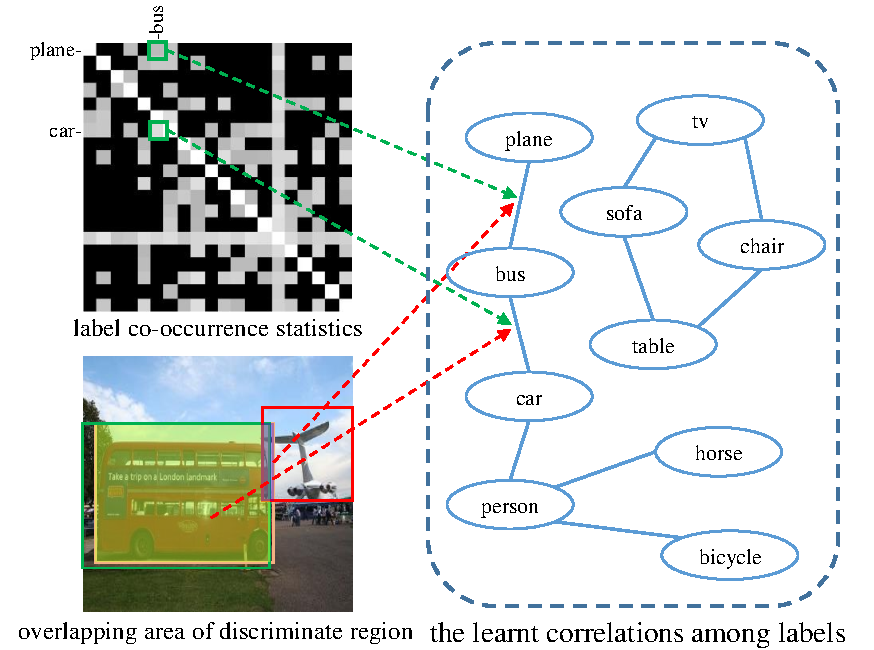
\includegraphics[width=1\linewidth]{fig_correlations.pdf}
    \end{center}
    \caption{There are two aspects involved in our label correlations: label co-occurrence based on statistics and overlapping area of discriminate region based on visual cues.}
    \label{fig:correlations}
\end{figure}

As an illustration, Figure \ref{fig:correlations} demonstrates the graphical description of label correlation model. Upper left shows co-occurrence matrix $A$ displaying the interaction between semantic concepts. The brighter the block is, the stronger the co-occurrence probability is. Bottom left illustrates an example of visual contextual clues, as known as overlapping area of discriminative regions. The larger the overlap is, the closer the labels pair correlation is.

Person, bicycle and house are three annotated semantic concept in this image, whose discriminative region is marked as bounding box in different color. The yellow box localizes the discriminative region of bicycle which is almost same to ground truth. The huge overlap between bicycle and person, strongly suggests the closer relationship between these two concepts, compared to rarely small overlap between bicycle and house. The figure on the right side clarifies the label correlation graph that integrates left two models. The interdependency of concepts pair is quantized on the edge between two label nodes. The bigger the value is, the higher the correlation is.

\textbf{Hierarchical Model and Spatial Constraints}
Considering the weakness of the single choice of segmentation, we utilize multiple segmentations to disambiguate low-level segmentation cues.
We divide the superpixels into different quantization level according to the particular segmentation scale we chose.
Then we include the inter-level energy cost $\phi_{inter}$ to investigate the most suitable segmentation scale each object belongs to.
Besides, we integrate the intra-level energy cost $\phi_{intra}$, which could discourage superpixel-level noise, to smooth the object boundaries.
Let the two neighboring superpixels (inter-level or intra-level) be $x_p$ and $x_q$ (\ie, $(p,q) \in \mathcal{N}$), we define the pairwise potential $\psi_{pq}$ as follows,
\begin{equation}
    \psi_{pq}(h_p,h_q) =
    \begin{cases}
        \phi_{inter}(h_p,h_q) &\mbox{ if } | l_p - l_q | = 1,
        \\
        \phi_{intra}(h_p,h_q) &\mbox{ if } l_p = l_q,
        \\
        0 &\mbox{ otherwise }
    \end{cases}
\end{equation}
where $l_p$ indicates the quantization level that the superpixel $x_p$ belongs to.
The inter-level energy cost $\phi_{inter}$ is defined as:
\begin{equation}
    \phi_{inter}(h_p,h_q) = \gamma \cdot O(x_p,x_q) \cdot \mathbf{1}(h_p \neq h_q)
\end{equation}
where $O(x_p,x_q)$ refers to the intersection (overlapping area) of two superpixels, $\mathbf{1}(\cdot)$ is the indicator function and $\gamma$ is the weighting coefficient.
This formulation is based on the higher order constraints \cite{kohli2009robust,ladicky2009associative} that superpixels lying within the same clique are more likely to take the same label.
And the intra-level energy cost $\phi_{intra}$ is defined as:
\begin{equation}
    \phi_{intra}(h_p,h_q) = S(x_p,x_q) \cdot (1-R(h_p,h_q))
\end{equation}
where $S(x_p,x_q) \in [0,1]$ measures the visual similarity between superpixel $x_p$ and $x_q$, $R(h_p,h_q) \in [0,1]$ is an inter-concept correlation between label $h_p$ and $h_q$.
Hence, we pay a high cost for the similar superpixels if they were assigned different labels and for the superpixels which were assigned an irrelevant label to the context.

\textbf{Label Consistency}
We require that the superpixel labels be consistent with the image labels: if any superpixel $x_p$ takes the label $i$, then image label indicator $y_i=1$; otherwise $y_i=0$. Such constraints can be encode by the following potential:
\begin{equation}
    \tau (\boldsymbol{y},\boldsymbol{h}) =
    C \cdot \sum_{i,p} \mathbf{1}(y_i=0 \land h_p=i)
\end{equation}
where $\mathbf{1}(\cdot)$ is the indicator function and $C$ is a positive constant that penalizes any inconsistency between the image-level and superpixel-level labels. It is worth noting that such label consistency potential is a soft constraint. Thus, we can further simultaneously refine superpxiel label and image label via an iterative process.

\subsection{Learning Parameters}
\label{learningparameters}
Due to the fact that pixel-level labels are not available during the training stage, we cannot use cross-validation \cite{kohli2009robust} to learn the weights for each potential.
Inspired by \cite{vezhnevets2011weakly}, we scale the pairwise potentials so as to make them comparable with unary potentials instead of using cross-validation procedure.
After selecting the weights of each potential, we can learn the parameters of appearance model $\boldsymbol{\theta_a}$ and latent semantic concept model $\boldsymbol{\theta_c}$ via an alternating optimization \cite{vezhnevets2011weakly}: 1) fix $\boldsymbol{h}$ and learn $\boldsymbol{\theta_a}$, $\boldsymbol{\theta_c}$; 2) fix $\boldsymbol{\theta_a}$, $\boldsymbol{\theta_c}$ and infer $\boldsymbol{h}$.
The first step corresponds to a continues optimization problem, hence the optimal appearance parameters $\boldsymbol{\theta_a}$ and latent semantic concept parameters $\boldsymbol{\theta_c}$ can be found efficiently via the existing supervised methods (\eg, \cite{shotton2006textonboost}). The second step is a discrete optimization problem and we provide the details in Section \ref{sec:inference}.

\begin{figure}[t]
    \begin{center}
        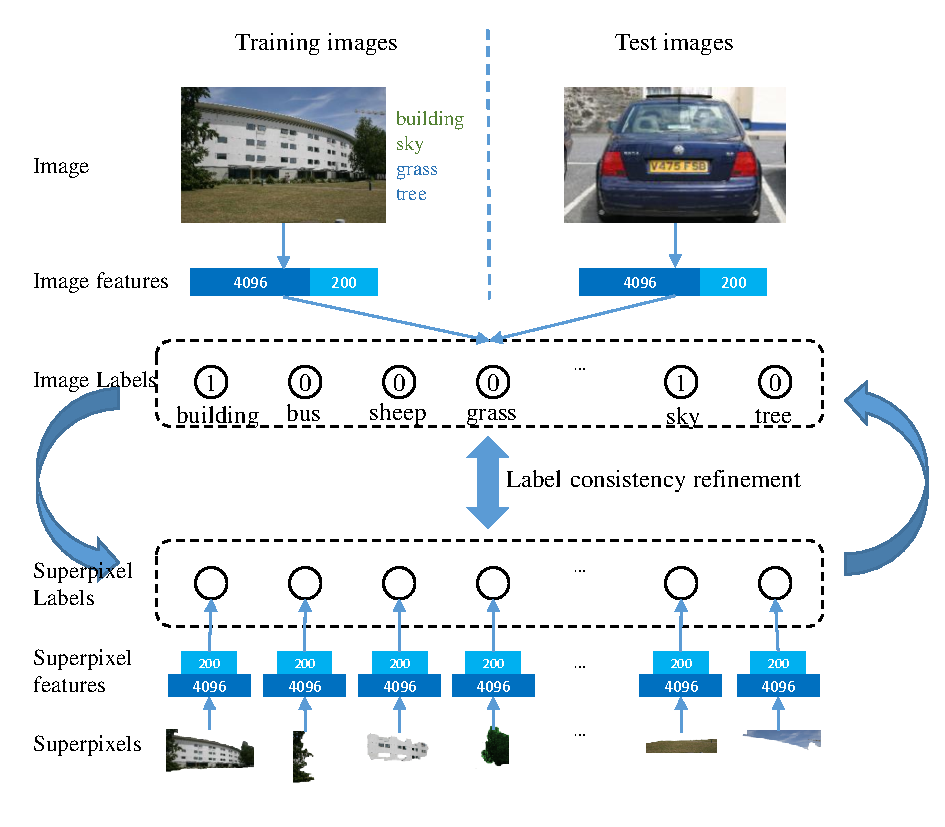
\includegraphics[width=1\linewidth]{fig_framework.pdf}
    \end{center}
    \vspace{-3mm}
    \caption{Illustration of our joint inference system. We simultaneously optimize the image-level label as well as superpixel-level label in a unified model so as to obtain the most suitable label configurations.}
    \label{fig:framework}
\end{figure}

\subsection{Joint Inference with Alternating Procedure}
\label{sec:inference}
Given an image $I$, our task is to assign each pixel a predefined semantic label.
We achieve this as an energy minimization problem \eqref{eq:energyfunction}, in which our inference algorithm searches for optimal configuration of image-level label $\boldsymbol{y}^\star$ and superpixel-level label $\boldsymbol{h}^\star$.
To efficiently minimize the energy function, we solve it in the following two alternating optimization steps, which can iteratively refine superpixel labels and image labels:
\begin{equation}
    \label{eq:binaryCRF}
    \begin{aligned}
        \boldsymbol{y}^* = \arg\min_{\boldsymbol{y}} &\sum_{i} {\varphi_{i}(y_i,\boldsymbol{I})} + \frac{1}{2} \tau(\boldsymbol{y},\boldsymbol{h}^*) \\ &+ \sum_{1 \le i,j \le L} {\varphi_{ij}(y_i,y_j)},
    \end{aligned}
\end{equation}
\begin{equation}
    \label{eq:multiclassCRF}
    \begin{aligned}
        \boldsymbol{h}^* = \arg\min_{\boldsymbol{h}} &\sum_{p} {\psi_{p}(h_p,\boldsymbol{x_p})} + \frac{1}{2} \tau(\boldsymbol{y}^*,\boldsymbol{h}) \\ &+ \sum_{(p,q) \in \mathcal{N}}{\psi_{pq}(h_p,h_q)}.
    \end{aligned}
\end{equation}
As a standard binary CRF problem, the first subproblem in Equation \eqref{eq:binaryCRF} has an explicit solution which utilizes min-cut/max-flow algorithms (\eg, the Dinic algorithm \cite{dinits1970algorithm}) to obtain the global optimal label configuration.
And the second subproblem in Equation \eqref{eq:multiclassCRF} reduces to an energy minimization for a multi-class CRF.
Although finding the global optimum for this energy function has been proved to be a NP-hard problem, there are various approximate methods for fast inference, such as approximate maximum a posteriori (MAP) methods (\eg, graph-cuts \cite{boykov2001fast}).
In this paper, we adopt move making approach \cite{boykov2001fast} that finds the optimal $\alpha$-expansion \cite{boykov2001fast,kolmogorov2004energy} by converting the problems into binary labeling  problems which can be solved efficiently using graph cuts techniques.
The energy obtain by $\alpha$-expansion has been proved to be within a known factor of the global optimum \cite{boykov2001fast}. Considering the two alternate optimization steps together, we summarize our joint inference system in Algorithm \ref{alg:energy}.


\renewcommand{\algorithmicrequire}{\textbf{Input:}}  % Use Input in the format of Algorithm
\renewcommand{\algorithmicensure}{\textbf{Output:}} % Use Output in the format of Algorithm

\begin{algorithm}
\caption{Energy Minimization Inference}
\label{alg:energy}
\begin{algorithmic}[1]
    \Require
    a image $I$ and its representation of superpixels $\{x_p\}$
    \Ensure
    the image-level label variables $\boldsymbol{y}$ and the superpixel-level label variables $\boldsymbol{h}$
    \State Construct the graphical model according to the energy function \eqref{eq:energyfunction}.
    \State Initialize $\boldsymbol{y}$ and $\boldsymbol{h}$ with the highest unary potential according to Equation \eqref{eq:global} and \eqref{eq:local}, respectively.
    \For{ iteration $t=1$ to $T$ }
        \State fix $\boldsymbol{y}$, optimize $\boldsymbol{h}$ via Equation \eqref{eq:multiclassCRF}
        \State fix $\boldsymbol{h}$, refine $\boldsymbol{y}$ via Equation \eqref{eq:binaryCRF}
    \EndFor
    \State Return the final configuration $\boldsymbol{y}$ and $\boldsymbol{h}$.
\end{algorithmic}
\end{algorithm}
